\documentclass[multi=tikzpicture,margin=0.25cm]{standalone}


\usepackage[utf8]{inputenc}
\usepackage[T1]{fontenc}

\usepackage{grafcet2}

\usetikzlibrary{circuits.plc.sfc}


\begin{document}


\begin{tikzpicture}[
		x=2.6\tikzcircuitssizeunit,
		y=1.3\tikzcircuitssizeunit,
		circuit plc grafcet,
	]
	\draw (0,0)
		to [flow direction] ++(0,-2)

		to [initstep={info=0,action={info=display}}] ++(0,-4)
		node [transition,info=b1 \& b0] (a) {}
		-- ++(0,-1)

		to [step={info={[red]1},info'={[blue]comment},
				action={
					info={[blue]hello},
					falling
				},
				action={
					info=G1\{init\},
					force
				},
				action={
					info=Ein sehr langer Text,
					condition=A \& B,
					falling
				},
				newrow,
				action={
					info={Test\_Text{=}1},
					condition={A{=}1 | Ä\_on}
				}
			}
		] ++(0,-4)

		-- ++(0,-4)
		to [macrostep={info=M0,info'=$\bullet$}] ++(0,-4)
		node [transition,info=b0] {}

		to [enclosingstep={info=S0}] ++(0,-4)
		node [transition,info=b0] {}

		to [step={info=2,
				action={info=bye,rising},
				action={info=bye,falling}
			}
		] ++(0,-4)
		node [transition={info=b1}] {}
		-- ++(0,-1) coordinate(split)

		(split) ++(-2,0) coordinate(n11)
		to [step={info=3.1}] ++(0,-4)
		node[transition]{}
		to [step={info=4.1}] ++(0,-4)
		node[transition]{}
		--++(0,-1)
		coordinate(n12)

		(split) ++(2,0) coordinate(n21)
		to [step={info=3.2}] ++(0,-4)
		node[transition]{}
		-- (n21 |- n12)
		coordinate(n22)

		(split) ++(6,0) coordinate(n31)
		to [step={info=33.3}] ++(0,-4)
		node[transition]{}
		to [step={info={\footnotesize 104.3}}] ++(0,-4)
		node[transition]{}
		-- (n31 |- n12)
		coordinate(n32)

		(n12) ++(2,0)
		|- ++(-8,-2)  |- (0,0)

		(n12) ++(2,-2)
		to [flow direction={info=to G2,pos=1}] ++(0,-2)
		%node[below]{to G2}

	;
	\draw[thick,double] (n11) ++(-0.5,0) -- (n31) --++(0.5,0) ;
	\draw[thick,double] (n12) ++(-0.5,0) -- (n32) --++(0.5,0) ;

\end{tikzpicture}

\begin{tikzpicture}[circuit plc grafcet,thick,y=1.5cm]
	\draw (0,0)
		to[initstep={info=0}] ++(0,-1)
		node[transition,info=start]{}
		|- ++(-1,-0.25)
		to[flow direction] (-1,0) -- (0,0)
	;
\end{tikzpicture}

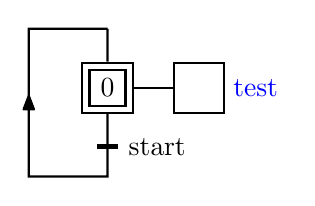
\begin{tikzpicture}[circuit plc sfc,thick,y=1.5cm]
	\draw (0,0)
		to[sfcstepi={info=0,sfcaction={info'={[blue]test}}}] ++(0,-1)
		node[sfctransition,info=start]{}
		|- ++(-1,-0.25)
		to[flow direction] (-1,0) -- (0,0)
	;
\end{tikzpicture}


\end{document}
